\chapter{Design}
\label{sec:design}
Aus den gesammelten Anforderungen vom \textbf{Kapitel \ref{sec:analyse}} wird es in diesem Kapitel um den Entwurf der Weboberfläche (WebUI) gehen. Die grundlegende Gestaltungsrichtlinie darunter die einheitliche Verwendung von Icons, Farben und Schriftgestaltung werden dabei beschrieben. Außerdem wird der Aufbau der zu entwickelnden Webanwendung mithilfe von Mockups dargestellt.\bigskip

\par
\begingroup
\leftskip=4em % Parameter anpassen
\rightskip\leftskip
\noindent \glqq Gutes Design ist so wenig Design wie möglich
Weniger Design ist mehr, konzentriert es sich doch auf das Wesentliche, statt die Produkte mit Überflüssigem zu befrachten. Zurück zum Puren, zum Einfachen!\grqq{} - Dieter Rams (vgl. 10 Thesen für gutes Design\footnote{\url{https://www.vitsoe.com/de/ueber-vitsoe/gutes-design}})
\par
\endgroup
\bigskip

\section{Gestaltungsrichtlinie}
\label{sec:gestaltungsrichtlinie}
Um der Webanwendung ein einheitliches, strukturiertes und benutzerfreundliches Design zu geben ist es erforderlich, feste Layoutvorgaben zu definieren. Sie sorgt für eine verständliche und intuitiv bedienbare Benutzeroberfläche, sodass eine positive Empfindung der Nutzer bei der Bedienung der Webanwendung hervorgerufen wird und ohne größere Einarbeitungszeit beherrscht werden kann. Diese Vorgabe wird auf alle Seiten der Webanwendung angewendet.

\subsection{Farben}
\label{subsec:farben}
Um die Webanwendung übersichtlich zu halten, wird auf die Verwendung mehrerer Farben verzichtet. Es werden grundsätzlich unbunte Farben verwendet, welche je nach Contentbereich in verschiedenen Intensitätsstufen zum Einsatz kommen. Die Gestaltung von Buttons und Daten werden wiederum mit bunten Farben gehalten, damit sie optisch auffallend sind.

\subsection{Schriftgestaltung}
\label{subsec:schriftgestaltung}
Bei der Schriftgestaltung, wie Schriftgröße und Schriftart, ist darauf zu achten, dass sie eine gute Lesbarkeit und ein modernes Aussehen bieten. Deshalb wird eine Schriftart verwendet, bei der es sich um eine serifenlose Schrift handelt.

\subsection{Icons}
\label{subsec:icons}
Die Buttons werden mit Icons integriert, um Inhalte schneller zu verstehen und den Nutzen der Funktionen zu verdeutlichen. Hierbei handelt es sich um allgemein übliche und bei mobilen Anwendung bekannte Icons. Sie sind so gewählt, dass sich der Nutzer bei den grundlegenden Funktionen auf der Webanwendung schnell zurechtfindet. Bei den Icons handelt es sich hierbei um keine Grafiken, sondern eine sogenannte Icon Fonts, welche über eigenes Stylesheet geladen werden. Die Fonts haben vor allem den Vorteil, dass sie auf jede Bildschirmgröße skaliert werden können. Für diese vorliegende Arbeit werden die Icon Fonts von Font Awesome\footnote{vgl. \url{https://fontawesome.com/}} verwendet.\bigskip

\begin{figure}[H]
  \begin{center}
    
\includegraphics[scale=0.5]{img/icons}
	\caption{Verwendete Icon Fonts} 
	\footnotesize\sffamily\textbf{Quelle:} \url{https://fontawesome.com/icons?d=gallery}  
	\label{fig:icons}
  \end{center}   
\end{figure}

\newpage
\section{Konzeption}
\label{sec:konzeption}
In diesem Abschnitt werden die erstellten Mockups, also die Wireframes der verschiedenen Seiten dargestellt und erläutert. Die definierte Gestaltungsrichtlinie sollte hierbei bei der Konzeption eingehalten werden.

\subsection{Mockup der Willkommensseite}
\label{subsec:mockup der willkommensseite}
Wenn die richtige URL aufgerufen wird, erscheint die Willkommensseite mit der Aufforderung zur Eingabe von Benutzernamen und Passwort \textbf{(Abbildung \ref{fig:mockup für die anmeldung})}. Zur Erinnerung, die Benutzerdaten werden in dieser Arbeit manuell in der Datenbank angelegt. Der Registrierungsvorgang wird in dieser Arbeit nicht vorhanden sein. Dieser wird für die zukünftige Weiterentwicklung festgehalten.\bigskip

Die Formulardaten werden über der Anmelden-Button verschickt, welcher ein Ereignis (Event) auslöst, um den richtigen User zu authentifizieren. Falls der User nicht existiert, wird eine Fehlermeldung auf der Seite ausgegeben \textbf{(Abbildung \ref{fig:mockup für die anmeldungsfehler})}.\bigskip

\begin{figure}[H]
	\centering
  \begin{minipage}[t]{0.45\linewidth}
  	    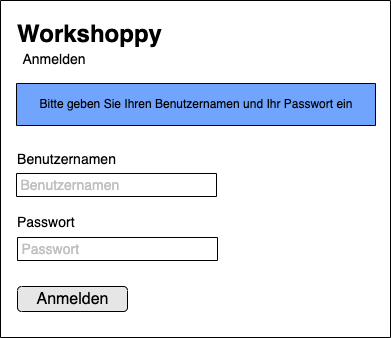
\includegraphics[width=.75\linewidth]{img/willkommenseite1}
		\caption{Mockup für die Anmeldung}
		\label{fig:mockup für die anmeldung}
  \end{minipage}
\hfill
  \begin{minipage}[t]{0.45\linewidth}
    	    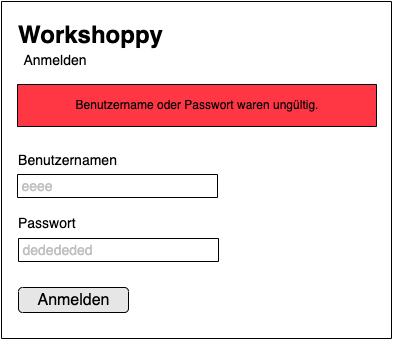
\includegraphics[width=.75\linewidth]{img/willkommenseite2}
		\caption{Mockup für die Anmeldungsfehler}
		\label{fig:mockup für die anmeldungsfehler}
  \end{minipage}
\end{figure}

\newpage
\subsection{Mockup der Hauptseite}
\label{subsec:mockup der hauptseite}
Nach der erfolgreichen Anmeldung wird der Nutzer, der für die Durchführung des Workshops verantwortlich ist, auf die Hauptseite weitergeleitet (Abbildung 4.3). Auf dieser Seite sind drei grundlegenden Bereiche (Nr.1, Nr.2 und Nr.3) zu sehen:\bigskip

\begin{figure}[H]
  \begin{center}
    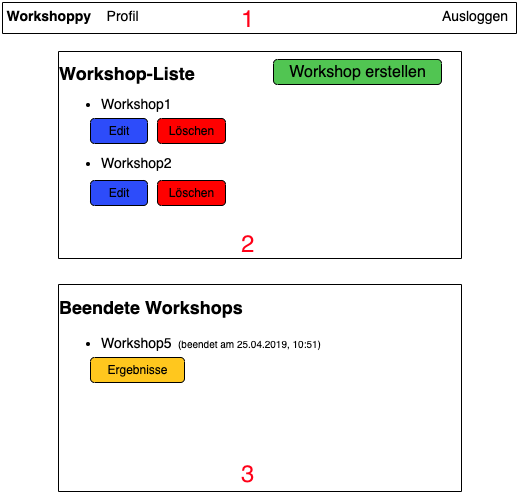
\includegraphics[scale=0.45]{img/hauptseite}
	\caption{Mockup der Hauptseite}  
	\label{fig:mockup für die hauptseite}
  \end{center}   
\end{figure}

\begin{enumerate}
\item Header:\\
Im Header befindet sich die Navigationsleiste. In dieser sind drei Navigationselemente enthalten.
\begin{itemize}
\item Workshoppy: \\
Navigiert den Nutzer zur Hauptseite. 
\item Profil:\\
Die angemeldete Person kann unter dem Profil seine Daten verwalten, wie z.B. seine Accountdaten (Benutzername, Passwort) ändern, den Account löschen und seine hinterlegten Personendaten anzeigen lassen.
\item Ausloggen:\\
Ermöglicht dem Nutzer, sich ordnungsgemäß von der Webanwendung auszuloggen.
\end{itemize}
\item Workshop-Liste:\\
In diesem Bereich werden die erstellten Workshops aufgelistet. Mit dem \glqq Workshop erstellen-Button\grqq{} kann ein neuer Workshop erstellt werden. Mit dem Edit- sowie Löschen-Button kann der Workshop gezielt bearbeitet und gelöscht werden.\bigskip

Die \textbf{Abbildung \ref{fig:workshop erstellen}} zeigt das Erstellen eines neuen Workshops. Der Titel ist ein Pflichtfeld und muss beim Erstellen angegeben werden. Als Option steht ein Textbereich für die Agenda zur Verfügung.\bigskip

\begin{figure}[H]
  \begin{center}
    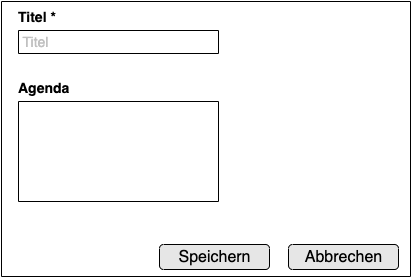
\includegraphics[scale=0.45]{img/workshop_erstellen}
	\caption{Mockup für das Erstellen eines neuen Workshops}  
	\label{fig:workshop erstellen}
  \end{center}   
\end{figure}

Beim Titel des Workshops handelt es sich um ein Linktext. Er ist klickbar und führt den Moderator beim Anklicken zur \textbf{Controller-Seite} des Workshops.
\item Beendete Workshops:\\
Sortieren nach Datum und Uhrzeit, werden die beendeten Workshops in diesem Bereich archiviert. Der Ergebnisse-Button führt zur \textbf{Ergebnisse-Seite} des archivierten Workshops.
\end{enumerate}

\newpage
\subsection{Mockup der Controller-Seite}
\label{subsec:mockup der controller-seite}
Jeder Workshop hat seine eigene Controller-Seite. Die \textbf{Abbildung \ref{fig:controller-seite}} zeigt beispielsweise die Controller-Seite von \glqq Workshops1\grqq{}. Auf dieser sind der Titel des Workshops (Nr.1), die Navigation-Tabs (Nr.2) und die Session-Liste (Nr.3) zu sehen.\bigskip

\begin{figure}[H]
  \begin{center}
    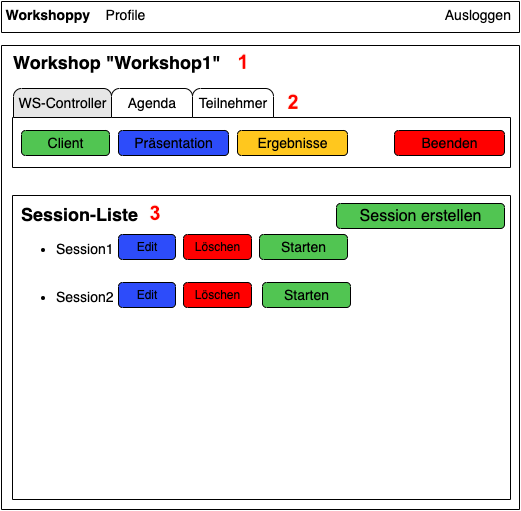
\includegraphics[scale=0.45]{img/controllerseite}
	\caption{Mockup der Controller-Seite}  
	\label{fig:controller-seite}
  \end{center}   
\end{figure}

Es sind drei Navigations-Tabs (Nr.2) vorhanden:
\begin{enumerate}
\item Das Navigation-Tab \glqq WS-Controller\grqq{} beinhaltet vier folgenden Buttons:
\begin{itemize}
\item Client-Button:\\
öffnet die \textbf{Teilnehmer-Seite} als neues Browser-Tab. Auf dieser Seite können die Teilnehmer die Dateneingabe tätigen.\bigskip

\textbf{Anmerkung:} Der Client-Button wird in der zukünftigen Weiterentwicklung entfernt, da der Moderator nicht für die Dateneingabe beteiligt werden darf. Für diese Arbeit wird der Client-Button aufgrund des Funktionstests erstmal erhalten bleiben.
\item Präsentation-Button:\\
öffnet als neues Browser-Fenster die \textbf{Präsentation-Seite}. Mittels Beamer präsentiert sie den Teilnehmern die eingegebenen Daten in Echtzeit.
\item Ergebnisse-Button:\\
öffnet neues Browser-Tab und ruft die \textbf{Ergebnisse-Seite} auf. Die Ergebnisse des Workshops werden dargestellt. Der Ergebnisse-Button ist erst aktiviert, wenn die Ergebnisse vorhanden sind.
\item Beenden-Button:\\
beendet den laufenden Workshop und leitet den Moderator zur \textbf{Hauptseite} weiter. Der Workshop wird anschließend in \glqq Beendete Workshops\grqq{} archiviert \textbf{(Abbildung \ref{fig:mockup für die hauptseite})}.
\end{itemize}
\item Die Agenda, falls sie vorhanden ist, wird im Navigation-Tab \glqq Agenda\grqq{} dargestellt.
\item Neben dem Einscannen des QR-Codes \textbf{(Abschnitt \ref{subsec:mockup der präsentation-seite})} können die Teilnehmer im Navigation-Tab \glqq Teilnehmer\grqq{} die Einladung per Mail senden lassen, um am Workshop teilzunehmen.\bigskip

\begin{figure}[H]
  \begin{center}
    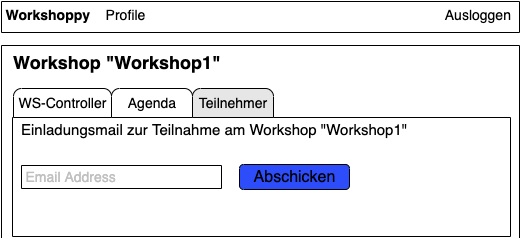
\includegraphics[scale=0.45]{img/einladungsmail}
	\caption{Mockup für das Navigation-Tab \glqq Teilnehmer\grqq{}}  
	\label{fig:mockup für einladungsmail}
  \end{center}   
\end{figure}
\end{enumerate}

Das Brainstorming wird in Session-Liste (Nr.3) in \textbf{Abbildung \ref{fig:controller-seite}} durchgeführt. Zunächst muss der Moderator mit dem \glqq Session Erstellen-Button\grqq{} eine neue Session anlegen \textbf{(Abbildung \ref{fig:mockup für das erstellen einer neuen session})}.\bigskip

\begin{figure}[H]
  \begin{center}
    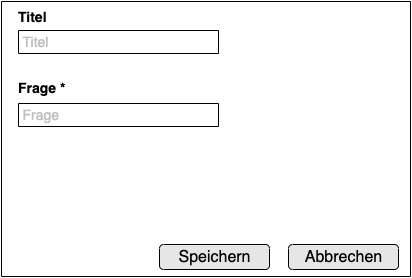
\includegraphics[scale=0.45]{img/session_erstellen}
	\caption{Mockup für das Erstellen einer neuen Session}  
	\label{fig:mockup für das erstellen einer neuen session}
  \end{center}   
\end{figure}

Die behandelte Frage, die auf der \textbf{Teilnehmer- und Präsentation-Seite} zu sehen sein wird, muss definiert werden. Als Option kann der Titel der Session angegeben werden. Wie viele Sessions in einem Workshop benötigt werden, das entscheidet der Moderator selbst. Er kann unbegrenzt viele Sessions erstellen.

Neben jeder Session sind in \textbf{Abbildung \ref{fig:controller-seite}} drei Buttons zu sehen. 
\begin{enumerate}
\item Edit-Button:\\
Mit ihm kann die Titel- sowie Fragenänderung durchgeführt werden.
\item Löschen-Button:\\
Der Löschen-Button löscht die Session inklusive der zugehörigen Ergebnisse.
\item Starten-Button:\\
Es wird erst \glqq gebrainstormt\grqq{}, wenn die Session gestartet ist. Während die Session läuft, darf sie nicht bearbeitet und gelöscht werden. Alle Buttons von nicht aktiven Sessions werden auch in dieser Phase deaktiviert. Es kann nur eine Session gestartet werden. Außerdem kann der Workshop bei laufender Session nicht beendet werden. Der \glqq Beenden-Button\grqq{} in WS-Controller \textbf{(Abbildung \ref{fig:controller-seite})} wird auch deaktiviert.\bigskip

Es gibt zusätzlich noch zwei weiteren Buttons, welche erst sichtbar werden, wenn eine Session gerade läuft. Das ist der \glqq Eingabe beenden-Button\grqq{} und \glqq Session Beenden-Button\grqq{} \textbf{(Abbildung \ref{fig:mockup für die aktive session})}.

\begin{figure}[H]
  \begin{center}
    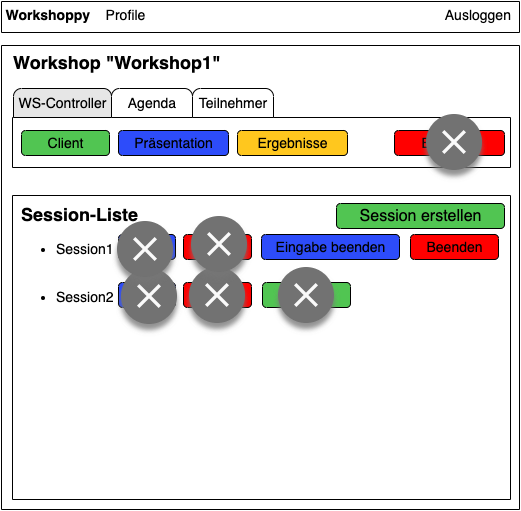
\includegraphics[scale=0.45]{img/session_ist_gestartet}
	\caption{Mockup für die aktive Session}  
	\label{fig:mockup für die aktive session}
  \end{center}   
\end{figure}

Der \glqq Eingabe beenden-Button\grqq{} bricht die Eingabefunktion auf der \textbf{Teilnehmer-Seite} ab. In dieser Situation können keine weiteren Daten mehr eingegeben werden. Der \glqq Session Beenden-Button\grqq{} beendet die gerade laufende Session. Erst nach dem Beenden einer laufenden Session werden alle zuvor deaktivierten Buttons wieder reaktiviert.
\end{enumerate}

\subsection{Mockup der Teilnehmer-Seite}
\label{subsec:Mockup der Teilnehmer-Seite}
Um auf diese Seite zu kommen, müssen die Teilnehmer entweder über Ihre Mobilgeräte den QR-Code auf der Präsentation-Seite \textbf{(Abschnitt \ref{subsec:mockup der präsentation-seite})} einscannen oder sie lassen sich die Einladung zur Teilnahme am Workshop per Mail zusenden, um am Workshop teilnehmen zu können. Die Teilnehmer-Seite stellt jedem Workshop-Teilnehmer die Dateneingabefunktion zu einer gestarteten Session bereit. Beim Aufrufen der Seite werden die Teilnehmer aufgefordert, einen Benutzernamen einzugeben \textbf{(Abbildung \ref{fig:mockup für eingabe der benutzernamen})}.

\begin{figure}[H]
  \begin{center}
    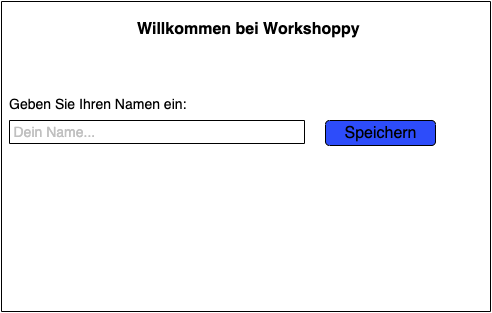
\includegraphics[scale=0.45]{img/teilnehmerseite}
	\caption{Mockup für Eingabe der Benutzernamen}  
	\label{fig:mockup für eingabe der benutzernamen}
  \end{center}   
\end{figure}

Nach Eingabe des Benutzernamens werden die Teilnehmer auf die Eingabefunktion weitergeleitet. Die \textbf{Abbildung \ref{fig:mockup für die anzeige der infotext}} beschreibt, dass die Teilnehmer-Seite gerade auf das Kommando des Moderators wartet. Sobald er eine Session startet, werden die Teilnehmer die Funktionen zur Dateneingabe freigeschaltet \textbf{(Abbildung \ref{fig:mockup für die eingabefunktion})}.

\begin{figure}[H]
	\centering
  \begin{minipage}[t]{0.45\linewidth}
  	    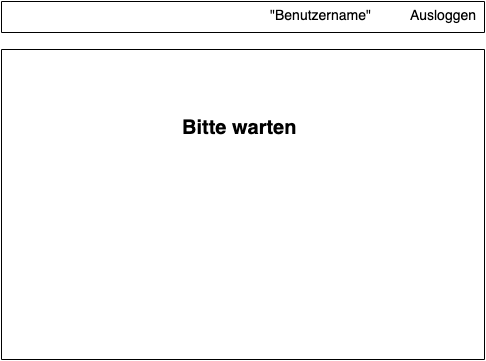
\includegraphics[width=.75\linewidth]{img/teilnehmerseite2}
		\caption{Mockup für die Anzeige der Infotext}
		\label{fig:mockup für die anzeige der infotext}
  \end{minipage}
\hfill
  \begin{minipage}[t]{0.45\linewidth}
    	    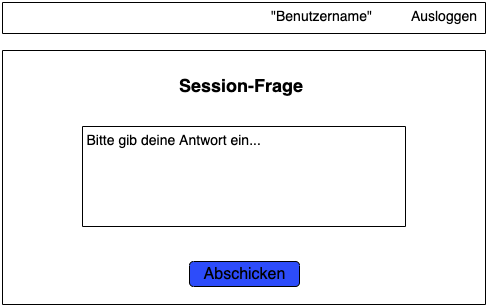
\includegraphics[width=.8\linewidth]{img/teilnehmerseite3}
		\caption{Mockup für die Eingabefunktion}
		\label{fig:mockup für die eingabefunktion}
  \end{minipage}
\end{figure}

In der Navigationsleiste in \textbf{Abbildung \ref{fig:mockup für die anzeige der infotext}} sowie in \textbf{Abbildung \ref{fig:mockup für die eingabefunktion}} sind zwei Navigationselemente zu sehen. Der Benutzername ist der Name des Teilnehmers, welcher zuvor eingegeben wurde. Das Ausloggen erlaubt dem Teilnehmer, seinen Benutzernamen zu ändern.\bigskip

Die Session-Frage in \textbf{Abbildung \ref{fig:mockup für die eingabefunktion}} ist die eigentliche Frage, welche in dieser Session behandelt wird. Die Textarea dient der Dateneingabe. Beim Klick auf den Abschicken-Button taucht die Dateneingabe sofort auf der \textbf{Präsentation-Seite} auf.

\subsection{Mockup der Präsentation-Seite}
\label{subsec:mockup der präsentation-seite}
Die Präsentation-Seite dient der Darstellung der Dateneingabe von allen Teilnehmern in Echtzeit. Die Seite hat zwei Zustände, nämlich passiv und aktiv.

\begin{itemize}
\item passiver Zustand:\\
Dieser Zustand bedeutet, dass keine Session gerade läuft. Die Präsentation-Seite zeigt bei diesem Zustand den QR-Code zur Teilnahme am Workshop an. Bevor die Session tatsächlich beginnt, können die Teilnehmer den QR-Code über Ihre Mobilgeräte einscannen, um am Workshop teilzunehmen \textbf{(Abbildung \ref{fig:mockup für das anzeigen des qr-codes})}. Falls es eine Agenda zu dem Workshop gibt, wird sie neben dem QR-Code dargestellt \textbf{(Abbildung \ref{fig:mockup für das anzeigen eines qr-code und einer agenda})}.\bigskip

\begin{figure}[H]
	\centering
  \begin{minipage}[t]{0.45\linewidth}
  	    \includegraphics[width=.8\linewidth]{img/präsentationseite1}
		\caption{Mockup für das Anzeigen eines QR-Codes}
		\label{fig:mockup für das anzeigen des qr-codes}
  \end{minipage}
\hfill
  \begin{minipage}[t]{0.45\linewidth}
    	    \includegraphics[width=.8\linewidth]{img/präsentationseite2}
		\caption{Mockup für das Anzeigen eines QR-Code und einer Agenda}
		\label{fig:mockup für das anzeigen eines qr-code und einer agenda}
  \end{minipage}
\end{figure}

\newpage
\item aktiver Zustand:\\
Die Präsentation-Seite befindet sich im aktiven Zustand, wenn die Session gestartet ist. Auf der Präsentation-Seite werden die Dateneingaben der Teilnehmer in Echtzeit präsentiert \textbf{(Abbildung \ref{fig:mockup für die darstellung der dateneingabe auf der präsentation-seite})}.\bigskip

\begin{figure}[H]
  \begin{center}
    \includegraphics[scale=0.5]{img/präsentationseite3}
	\caption{Mockup für die Darstellung der Dateneingabe auf der Präsentation-Seite}  
	\label{fig:mockup für die darstellung der dateneingabe auf der präsentation-seite}
  \end{center}   
\end{figure}

Die behandelte Frage (Nr.1) ist am oberen Inhaltsbereich zu sehen. Die Eingaben der Teilnehmer (Nr.2) werden wie ein Notizzettel visualisiert. Ein Notizzettel besteht aus zwei Teilen, dem Namen des Teilnehmers und seine Idee. Am unteren Bereich der Präsentation-Seite befinden sich zwei Buttons (Nr.3). Während die Session läuft, kann der QR-Code des Workshops mit dem Drücken des QR-Code-Buttons angezeigt werden. Wenn der QR-Code-Button getätigt wird, wandelt er sich anschließend im \glqq QR-Code ausblenden-Button\grqq{} um. Die Session wird dabei nicht beendet und kann mit dem Drücken des \glqq QR-Code ausblenden-Button\grqq{} wieder, wie auf der \textbf{Abbildung \ref{fig:mockup für die darstellung der dateneingabe auf der präsentation-seite}}, zurückkommen. Der QR-Code kann sowohl im passiven Zustand \textbf{(Abbildung \ref{fig:mockup für das anzeigen des qr-codes})} als auch im aktiven Zustand dargestellt werden. Der Vollbild-Button wandelt die Präsentation-Seite in den Vollbildmodus um.\bigskip

Um die eingegebenen Daten auf der Präsentation-Seite zusammenfassen zu können, muss der Moderator den \glqq Eingabe beenden-Button\grqq{} auf der \textbf{Controller-Seite}, wie in \textbf{Abbildung \ref{fig:mockup für die aktive session}} zu sehen ist, drücken. Die Kategorien lassen sich anschließend mit dem \glqq Kategorie erstellen-Button\grqq{} erstellen \textbf{(Abbildung \ref{fig:mockup für zusammenfassung-modus auf der präsentation-seite})}.

\begin{figure}[H]
  \begin{center}
    \includegraphics[scale=0.5]{img/präsentationseite4}
	\caption{Mockup für Zusammenfassung-Modus auf der Präsentation-Seite}  
	\label{fig:mockup für zusammenfassung-modus auf der präsentation-seite}
  \end{center}   
\end{figure}

Direkt auf der Präsentation-Seite kann der Moderator die Daten mit der Drag-\&-Drop-Funktion in Kategorien zusammenfassen. Die Kategorien selbst lassen sich nicht verschieben. Das Löschen einer Kategorie erfolgt mit dem Klick auf dem X-Button. Es wird nur die Kategorie gelöscht, d.h. die darin befindlichen Daten bleiben auf der Präsentation-Seite erhalten.
\end{itemize}

\subsection{Mockup der Ergebnisse-Seite}
\label{subsec:mockup der ergebnisse-seite}
Mit Klick auf den Ergebnisse-Button in \textbf{Abbildung \ref{fig:mockup für die hauptseite}} sowie in \textbf{Abbildung \ref{fig:controller-seite}} wird als neues Browser-Tab die Ergebnisse-Seite des Workshops geöffnet. Auf der Seite befinden sich die Daten inklusive Kategorien des Workshops. Die Ergebnisse-Seite beinhaltet außerdem einen Button, mit dem die Ergebnisse als eine PDF-Datei heruntergeladen werden kann \textbf{(Abbildung \ref{fig:mockup für die darstellung der ergebnisse des workshops})}.

\begin{figure}[H]
  \begin{center}
    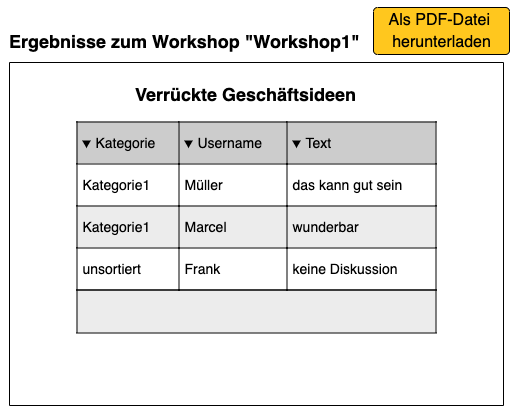
\includegraphics[scale=0.45]{img/ergebnisse_seite}
	\caption{Mockup für die Darstellung der Ergebnisse des Workshops}  
	\label{fig:mockup für die darstellung der ergebnisse des workshops}
  \end{center}   
\end{figure}

